\icode{N18I-EXM-FI-L2-260625-001}
\nceeID[5]{2018新课标\Rmnum{1}}{22}
如图(\(a\))，一弹簧上端固定在支架顶端，下端悬挂一托盘；一标尺由游标和主尺构成，主尺竖直固定在弹簧左边；托盘上方固定有一能与游标刻度线准确对齐的装置，简化为图中的指针。
	
	现要测量图(\(a\))中弹簧的劲度系数。当托盘内没有砝码时，移动游标，使其零刻度线对准指针，此时标尺读数为\,\qty{1.950}{cm}；当托盘内放有质量为\,\qty{0.100}{kg}的砝码时，移动游标，再次使其要刻度线对准指针，标尺示数如图(\(b\))所示,其读数为\underline{\hbox to 4em{}}\,\qty{}{cm}。当地的重力加速度大小为\,\qty{9.80}{m/s^2}，此弹簧的劲度系数为\underline{\hbox to 4em{}}\,\qty{}{N/m}(保留3位有效数字)。

	\begin{tikzpicture}
		\draw (1.5,0) rectangle(1.6,5.3);
		\draw (.75,5) rectangle(1.7,5.05);
		\filldraw[fill=white] (1.45,4.95) rectangle(1.65,5.1);
		\draw (0,0) rectangle(.3,3);
		\filldraw[fill=white] (-.1,2.2) rectangle(.1,2.45);
		\filldraw[fill=gray] (-.3,-.2) rectangle(.6,0);
		\filldraw[fill=gray] (1.3,-.2) rectangle(1.8,.2);
		\draw[gray] (-.6,-.2)--(2.2,-.2);
		\foreach \x in {-.5,-.2,...,2}
			\draw[gray] (\x,-.4)--++(.2,.2);
		\foreach \y in {4,3.6,...,2.8}
			\draw (.7,\y)--++(.4,.2);
		\foreach \y in {3.8,3.4,...,2.6}
			\draw (1.1,\y)--++(-.4,.2);
		\draw (.7,2.8)--(.9,2.7)--(.9,2)--(.6,1.8)--(1.2,1.8)--(.9,2);
		\draw (1.1,4.2)--(.9,4.3)--(.9,5);
		\draw[->,red,thick] (1.2,2.4)--(.1,2.4);
		\fill (.9,2.4) circle(.05);
		\draw (-.3,.5)node[left]{\footnotesize 主尺}--(.1,1);
		\draw (-.3,2)node[left]{\footnotesize 游标}--(0,2.3);
		\draw (.15,4)node[above]{\footnotesize 指针}--(.6,2.5);
	\end{tikzpicture}
	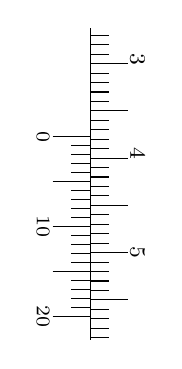
\begin{tikzpicture}[scale=1.2]
		\foreach \y in {-.95,-.855,...,.95}
			\draw (-.2,\y)--(0,\y);
		\foreach \y in{-.95,-.475,...,.95}
			\draw (-.4,\y)--(0,\y);
		\foreach \y/\n in {.95/0,0/10,-.95/20}
			\node at(-.5,\y)[rotate=-90]{\scriptsize\(\n\)};
		\foreach \y in {-1.175,-1.075,...,2.075}
			\draw (0,\y)--(.2,\y);
		\foreach \y in {-.775,-.275,...,1.875}
			\draw (0,\y)--(.4,\y);
		\foreach \y/\n in {-.275/5,.775/4,1.775/3}
			\node at(.5,\y)[rotate=-90]{\footnotesize\(\n\)};
		\draw (0,2.1)--(0,-1.2);
	\end{tikzpicture}